\title{CS4221/CS5421}

\subtitle{Tutorial 4: Normal Forms and Normalisation}

\author{Mark Meng Huasong}

\institute[National University of Singapore] % (optional, but mostly needed)
{
	School of Computing\\
	National University of Singapore
}

\titlegraphic{
	
\includegraphics[width=2cm]{nus-logo}
}

\date{Week 6, 2022 Spring}

\begin{frame}
	\titlepage
	\begin{tcolorbox}
		\begin{center}
			{\scriptsize \textcolor{red}{All the materials within presentation slides are protected by copyrights.\\
					It is forbidden by NUS to upload these materials to the Internet.}}
		\end{center}
	\end{tcolorbox}
\end{frame}

\begin{comment}
\begin{frame}
	Updated on 9 Oct (Saturday):
	\begin{itemize}
		\item Fixed a FD missing in $R_1$ of Q4(e) in page 29.\\
		i.e., replaced $\Sigma_1 = \{\{A\} \rightarrow \{C\}, \{B\} \rightarrow \{A\}, \{C\} \rightarrow \{D\}\}$ with $\Sigma_1 = \{\{A\} \rightarrow \{C\}, \{A\} \rightarrow \{B\},\{B\} \rightarrow \{A\}, \{C\} \rightarrow \{D\}\}$.
	\end{itemize}
\end{frame}
\end{comment}

\begin{frame}[fragile]{Question 1(a) Preliminary}

Consider the relations $R=\{A, B, C, D, E\}$ with the set of functional dependencies $\Sigma=\{\{A\} \rightarrow \{A, B, C\}, \{A, B\} \rightarrow \{A\}, \{B, C\} \rightarrow \{A, D\}, \{B\} \rightarrow \{A, B\}, \{C\} \rightarrow \{D\}\}$.\\\vspace{5pt}

(a) What preliminary work is needed to study the normalization of $R$ with $\Sigma$? \vspace{15pt}

\textbf{Solution}: Attribute closure, candidate keys \& prime attributes, and compact minimal cover\vspace{5pt}

\textbf{Explanation}: To determine the \textbf{norm form}, you need to know which attribute(s) is/are \textit{\textbf{prime}}. You also need to identify \textbf{\textit{superkeys}}, too. Therefore you need to compute the \textbf{\textit{attribute closure}} at first.\\\vspace{5pt}

To perform \textbf{BCNF decomposition} or \textbf{3NF synthesise} (definitely you'll be asked to do that), you need to have a \textbf{\textit{compact minimal cover}} on hands.

\end{frame}

\begin{frame}[fragile]{Question 1 (a) Cont.}
Let's compute the attribute closures of the attributes in $R$ with $\Sigma$ in order to find the candidate keys of $R$ with $\Sigma$. \vspace{15pt}

The original question is:\\ $\Sigma=\{\{A\} \rightarrow \{A, B, C\}, \{A, B\} \rightarrow \{A\}, \{B, C\} \rightarrow \{A, D\}, \{B\} \rightarrow \{A, B\}, \{C\} \rightarrow \{D\}\}$.\\\vspace{5pt} 

\begin{columns}[t]
	\column{0.45\textwidth}
	\textcolor{gray}{\scriptsize \textit{(Let's start with single attribute first)}}\\
	$\{A\}^{+}= \{A, B, C, D\}$\\	
	$\{B\}^{+}= \{A, B, C, D\}$\\	
	$\{C\}^{+}= \{C, D\}$\\
	$\{D\}^{+}= \{D\}$\\
	$\{E\}^{+}= \{E\}$\\ \vspace{5pt}
	\textcolor{gray}{\textit{\scriptsize (Two attributes' combination)}}\\
	$\{A, B\}^{+}= \{A, B, C, D\}$\\
	$\{A, C\}^{+}= \{A, B, C, D\}$\\
	$\{A, D\}^{+}= \{A, B, C, D\}$
	\column{0.45\textwidth}	
	$\underline{\{A, E\}^{+}}= \{A, B, C, D, E\}$\\
	$\{B, C\}^{+}= \{A, B, C, D\}$\\
	$\{B, D\}^{+}= \{A, B, C, D\}$\\
	$\underline{\{B, E\}^{+}}= \{A, B, C, D, E\}$\\
	$\{C, D\}^{+}= \{C, D\}$\\
	$\{C, E\}^{+}= \{C, D, E\}$\\
	$\{D, E\}^{+}= \{D, E\}$\\ \vspace{5pt}
	Other attribute closures need not be computed.
\end{columns}
\end{frame}

\begin{frame}[fragile]{Question 1 (a) Cont.}
	The candidate keys are $\{A, E\}$ and $\{B, E\}$. \\\vspace{10pt}
	The prime attributes are $A$, $B$ and $E$.\\ \vspace{10pt}
	Superkeys include  $\{A, E\}$, $\{B, E\}$, $\{A, B, E\}$, $\{A, C, E\}$, $\{B, C, E\}$ , $\{A, D, E\}$, $\{B, D, E\}$, $\{A, B, C, E\}$, $\{A, C, D, E\}$, $\{A, B, D, E\}$, $\{B, C, D, E\}$ and $\{A, B, C, D, E\}$.\\ \vspace{15pt}
	\begin{figure}
		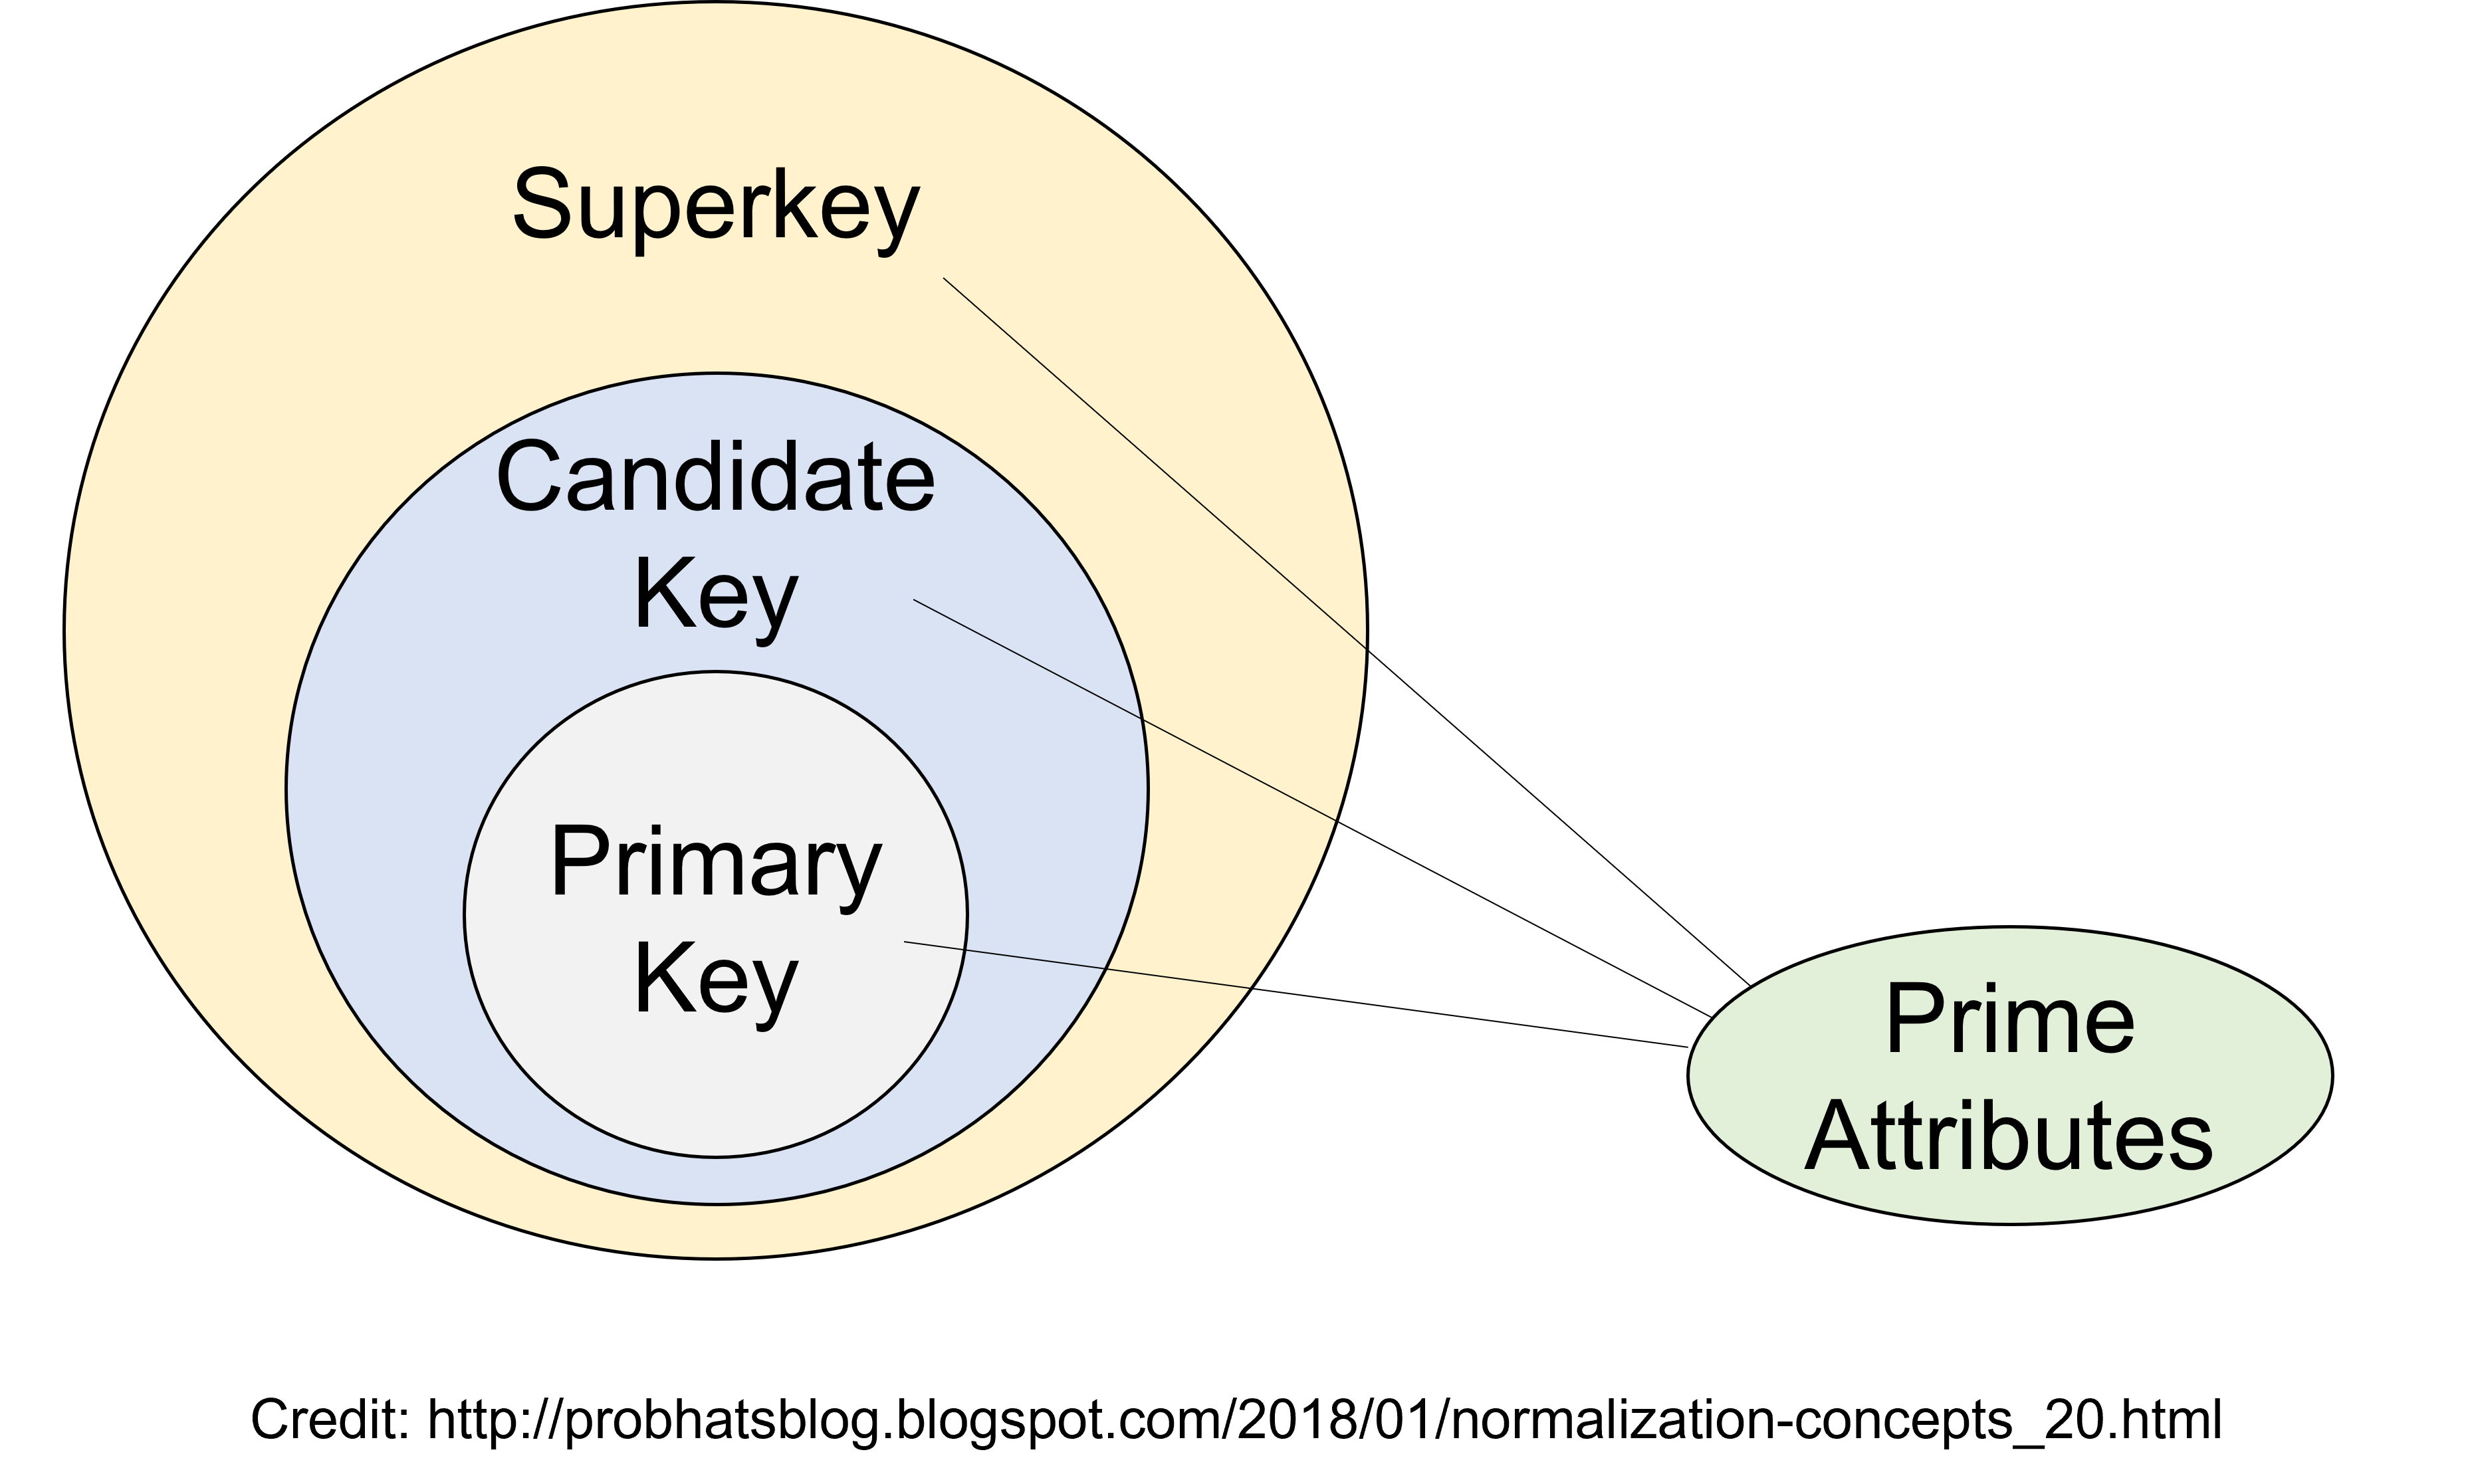
\includegraphics[width=0.6\textwidth, trim=0 0 0 0, clip]{t5/images/keys.png}
	\end{figure}
\end{frame}

\begin{frame}[fragile]{Question 1 (a) Cont.}
	Now let's compute a minimal cover of $R$ with $\Sigma$.\vspace{10pt}
	
	We start from $\Sigma$: \\\vspace{5pt}
	$\{A\} \rightarrow \{A, B, C\}$\\
	$\{A, B\} \rightarrow \{A\}$\\
	$\{B, C\} \rightarrow \{A, D\}$\\
	$\{B\} \rightarrow \{A, B\}$\\
	$\{C\} \rightarrow \{D\}$\\\vspace{5pt}
	Step 1, we simplify the right-hand sides:\\\vspace{3pt}
	\begin{columns}[t]
	\column{0.45\textwidth}
	$\{A\} \rightarrow \{A\}$\\
	$\{A\} \rightarrow \{B\}$\\
	$\{A\} \rightarrow \{C\}$\\
	$\{A, B\} \rightarrow \{A\}$\\
	$\{B, C\} \rightarrow \{A\}$
	\column{0.45\textwidth}
	$\{B, C\} \rightarrow \{D\}$\\
	$\{B\} \rightarrow \{A\}$\\
	$\{B\} \rightarrow \{B\}$\\
	$\{C\} \rightarrow \{D\}$
	\end{columns}
\end{frame}

\begin{frame}[fragile]{Question 1 (a) Cont.}
	Step 2, we simplify the left-hand sides:\\\vspace{3pt}
	$\{A\} \rightarrow \{A\}$.\\	
	$\{A\} \rightarrow \{B\}$.\\	
	$\{A\} \rightarrow \{C\}$.\\	
	$\{A,\cancel{B}\} \rightarrow \{A\}$ because $\{A\} \rightarrow \{A\}$.\\	
	$\{B, \cancel{C}\} \rightarrow \{A\}$ because $\{B\} \rightarrow \{A\}$.\\	
	$\{B, \cancel{C}\} \rightarrow \{D\}$ because $\{B\} \rightarrow \{D\}$ \\\vspace{3pt}
	(we could also remove $\{\cancel{B}, C\} \rightarrow \{D\}$ because $\{C\} \rightarrow \{D\}$). Note that we know that $\{B\} \rightarrow \{D\}$ because $\{B\}^{+}= \{A, B, C, D\}$.\\\vspace{3pt}
	$\{B\} \rightarrow \{A\}$.\\
	$\{B\} \rightarrow \{B\}$.\\
	$\{C\} \rightarrow \{D\}$.
\end{frame}

\begin{frame}[fragile]{Question 1 (a) Cont.}
	Step 3, we simplify the set:\\\vspace{3pt}
	$\cancel{\{A\} \rightarrow \{A\}}$ because it is trivial.\\	
	$\{A\} \rightarrow \{B\}$.\\	
	$\{A\} \rightarrow \{C\}$.\\	
	$\{B\} \rightarrow \{A\}$.\\	
	$\cancel{\{B\} \rightarrow \{D\}}$ because it can be derived from the others.\\	
	$\cancel{\{B\} \rightarrow \{B\}}$ $\cancel{\{A\} \rightarrow \{A\}}$.\\	
	$\{C\} \rightarrow \{D\}$.\\\vspace{5pt}
	
	\textbf{The result is:} \\\vspace{3pt}
	$\{A\} \rightarrow \{B\}$\\	
	$\{A\} \rightarrow \{C\}$\\	
	$\{B\} \rightarrow \{A\}$\\
	$\{C\} \rightarrow \{D\}$
\end{frame}

\begin{frame}[fragile]{Question 1 (a) Cont.}
	\begin{alertblock}{Notice}
	Note that there can be other minimal covers that the algorithm can compute by considering the functional dependencies in a different order at each step of the algorithm. This is not the case in the example.
	\end{alertblock}\vspace{5pt}

	However, there is a minimal cover that the algorithm cannot compute:\\\vspace{5pt}
	$\{A\} \rightarrow \{B\}$\\
	$\{B\} \rightarrow \{A\}$\\
	$\{B\} \rightarrow \{C\}$\\
	$\{C\} \rightarrow \{D\}$\\\vspace{10pt}	
	If the algorithm starts from $\Sigma^{+}$, then it can find all minimal covers.
\end{frame}

\begin{frame}[fragile]{Question 1 (a) Cont.}
	Next, let's compute a compact minimal cover of $R$ with $\Sigma$.\vspace{10pt}
	
	Given the minimal cover of $R$ with $\Sigma$:\\\vspace{3pt}
	$\{A\} \rightarrow \{B\}$\\	
	$\{A\} \rightarrow \{C\}$\\	
	$\{B\} \rightarrow \{A\}$\\
	$\{C\} \rightarrow \{D\}$\\\vspace{5pt}
	The \textbf{compact minimal cover} is:\\\vspace{3pt}
	$\{A\} \rightarrow \{B, C\}$\\	
	$\{B\} \rightarrow \{A\}$\\	
	$\{C\} \rightarrow \{D\}$
\end{frame}

\begin{frame}[fragile]{Question 1 (a) Cont.}
Now let's look back the relation $R$ with all FDs ($\Sigma$) \textcolor{red}{\textbf{with this un-official visualization}}:\\\vspace{5pt}
\begin{figure}
	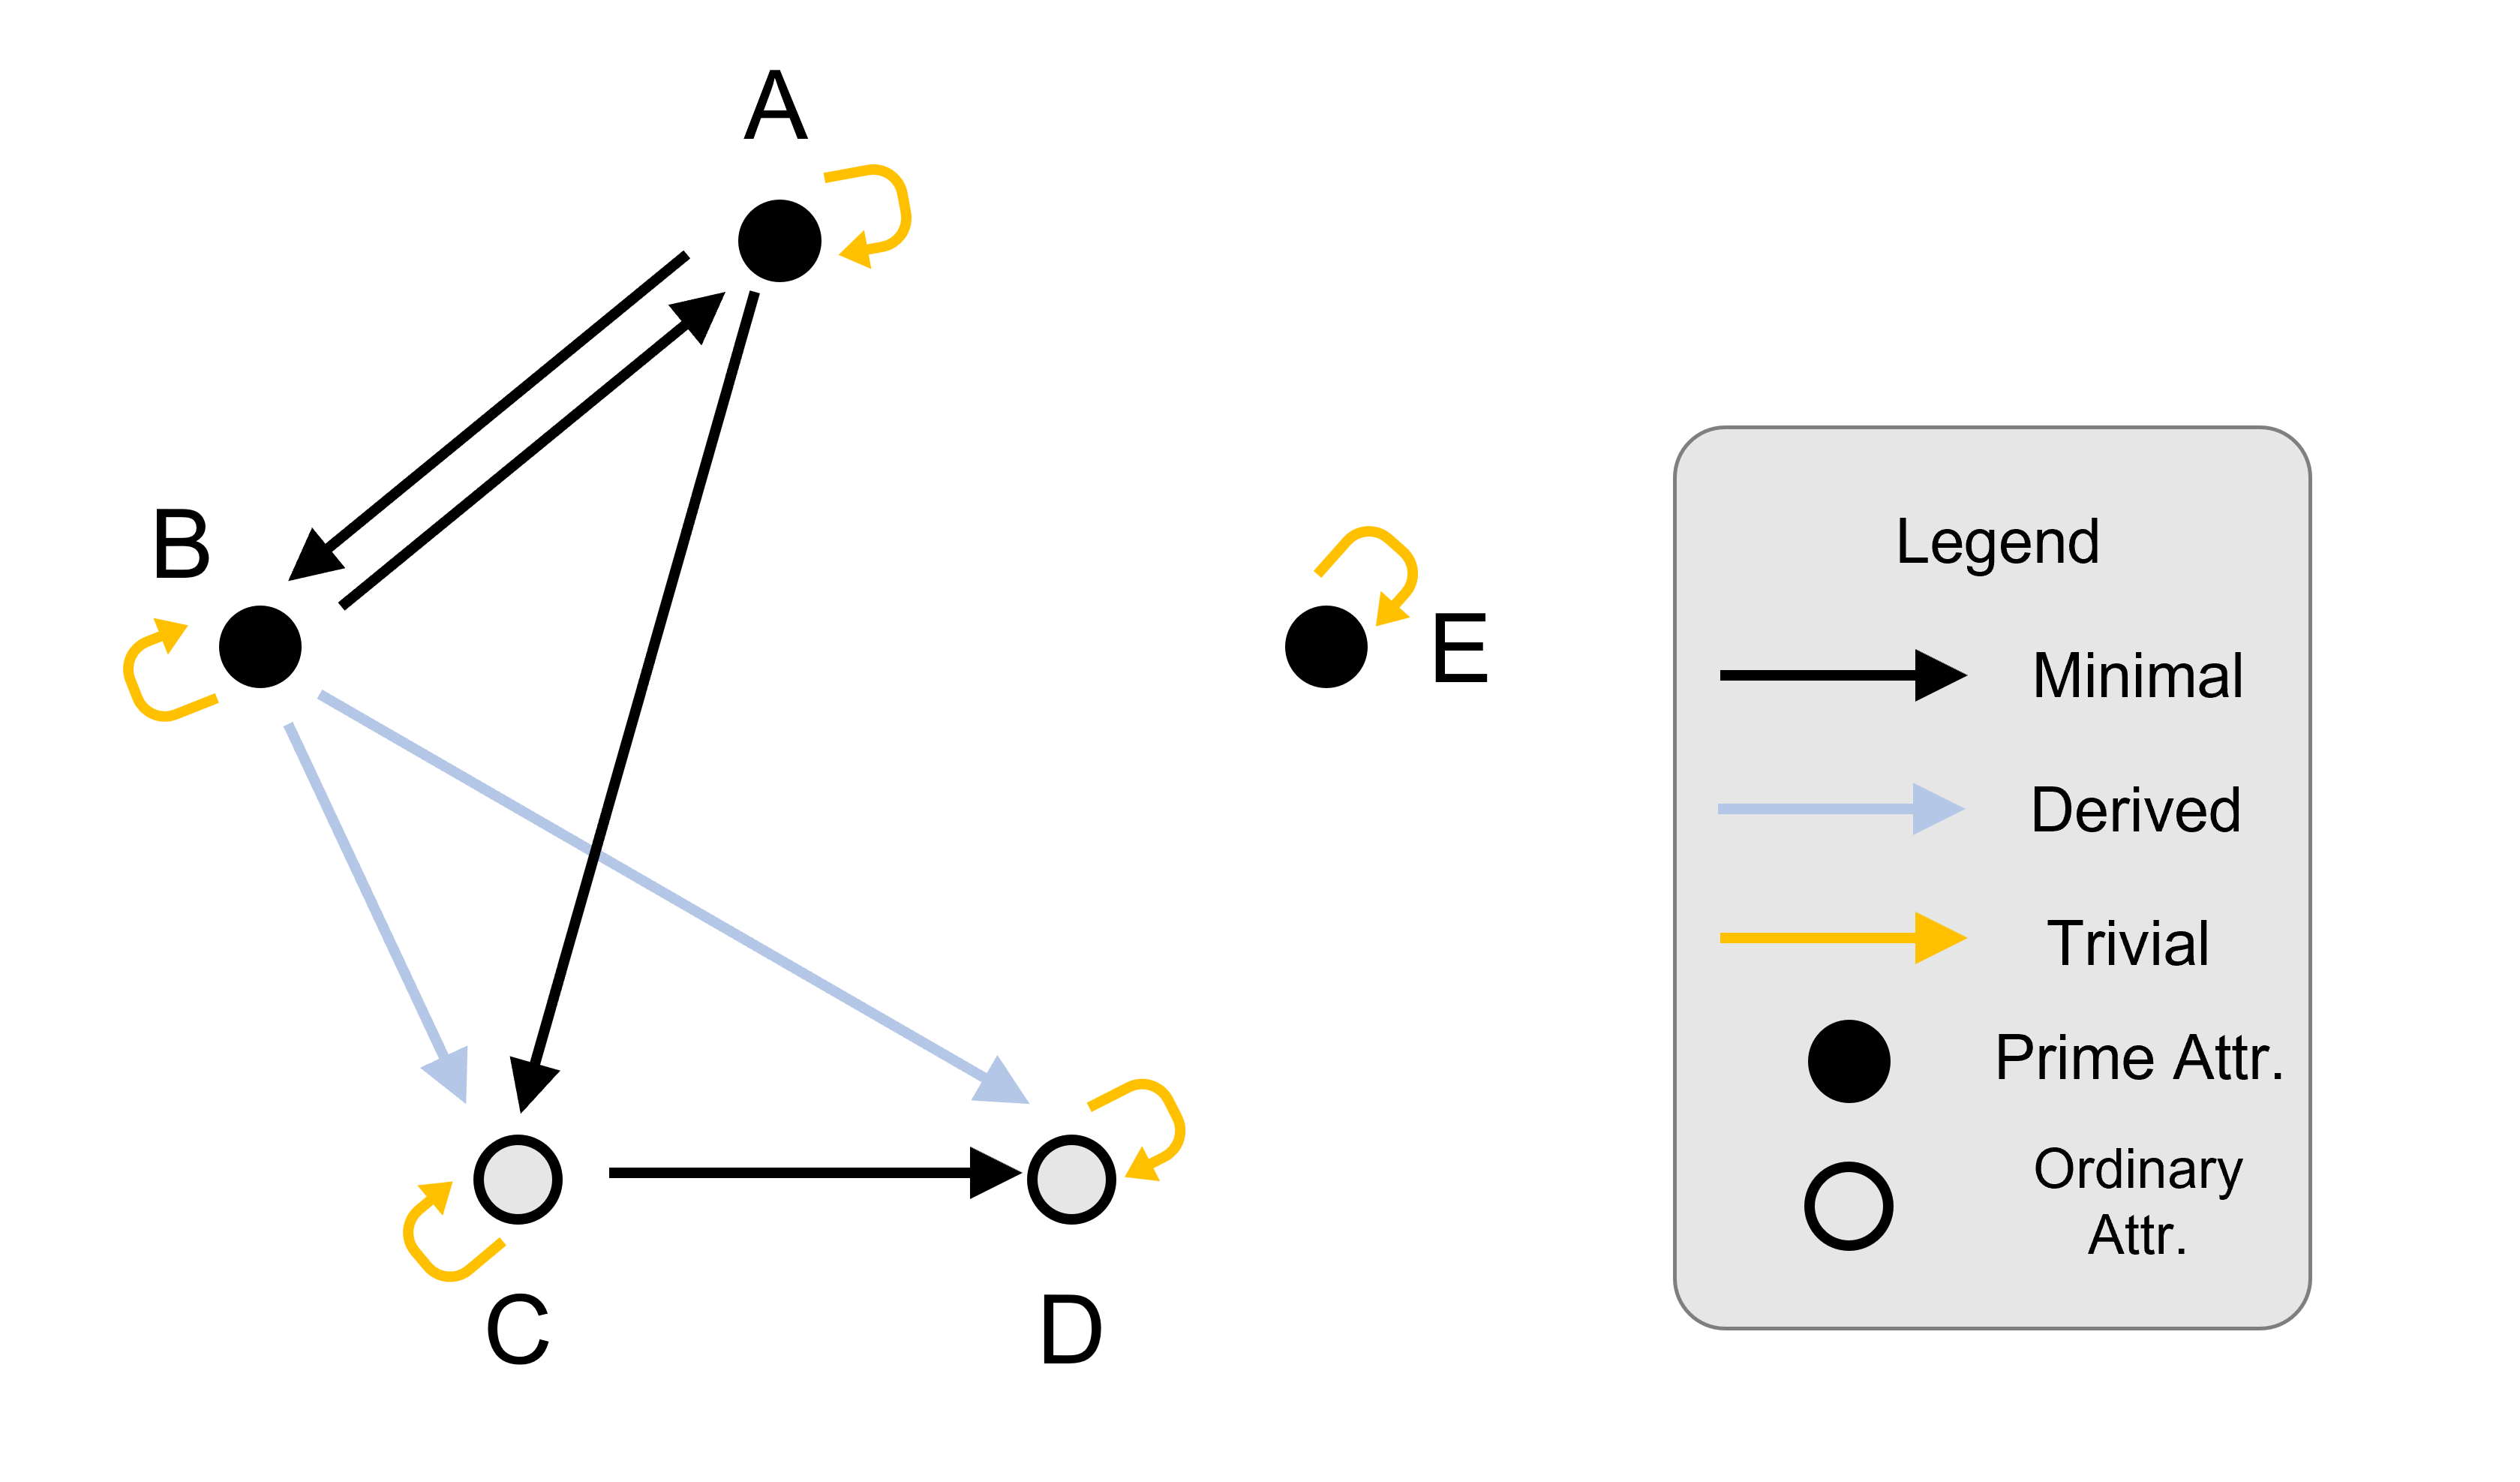
\includegraphics[width=0.85\textwidth, trim=0 0 0 0, clip]{t5/images/end_q1.png}
\end{figure}

\textit{(We will keep using this (kind of) figures for later demonstrations)}
\end{frame}

\begin{frame}[fragile]{Question 1 (b-c) Normal Forms}
(*) Is $R$ with $\Sigma$ in 2NF? (Just for recap purpose)\\
(b) Is $R$ with $\Sigma$ in 3NF?\\
(c) Is $R$ with $\Sigma$ in BCNF?\\\vspace{10pt}

\begin{figure}
	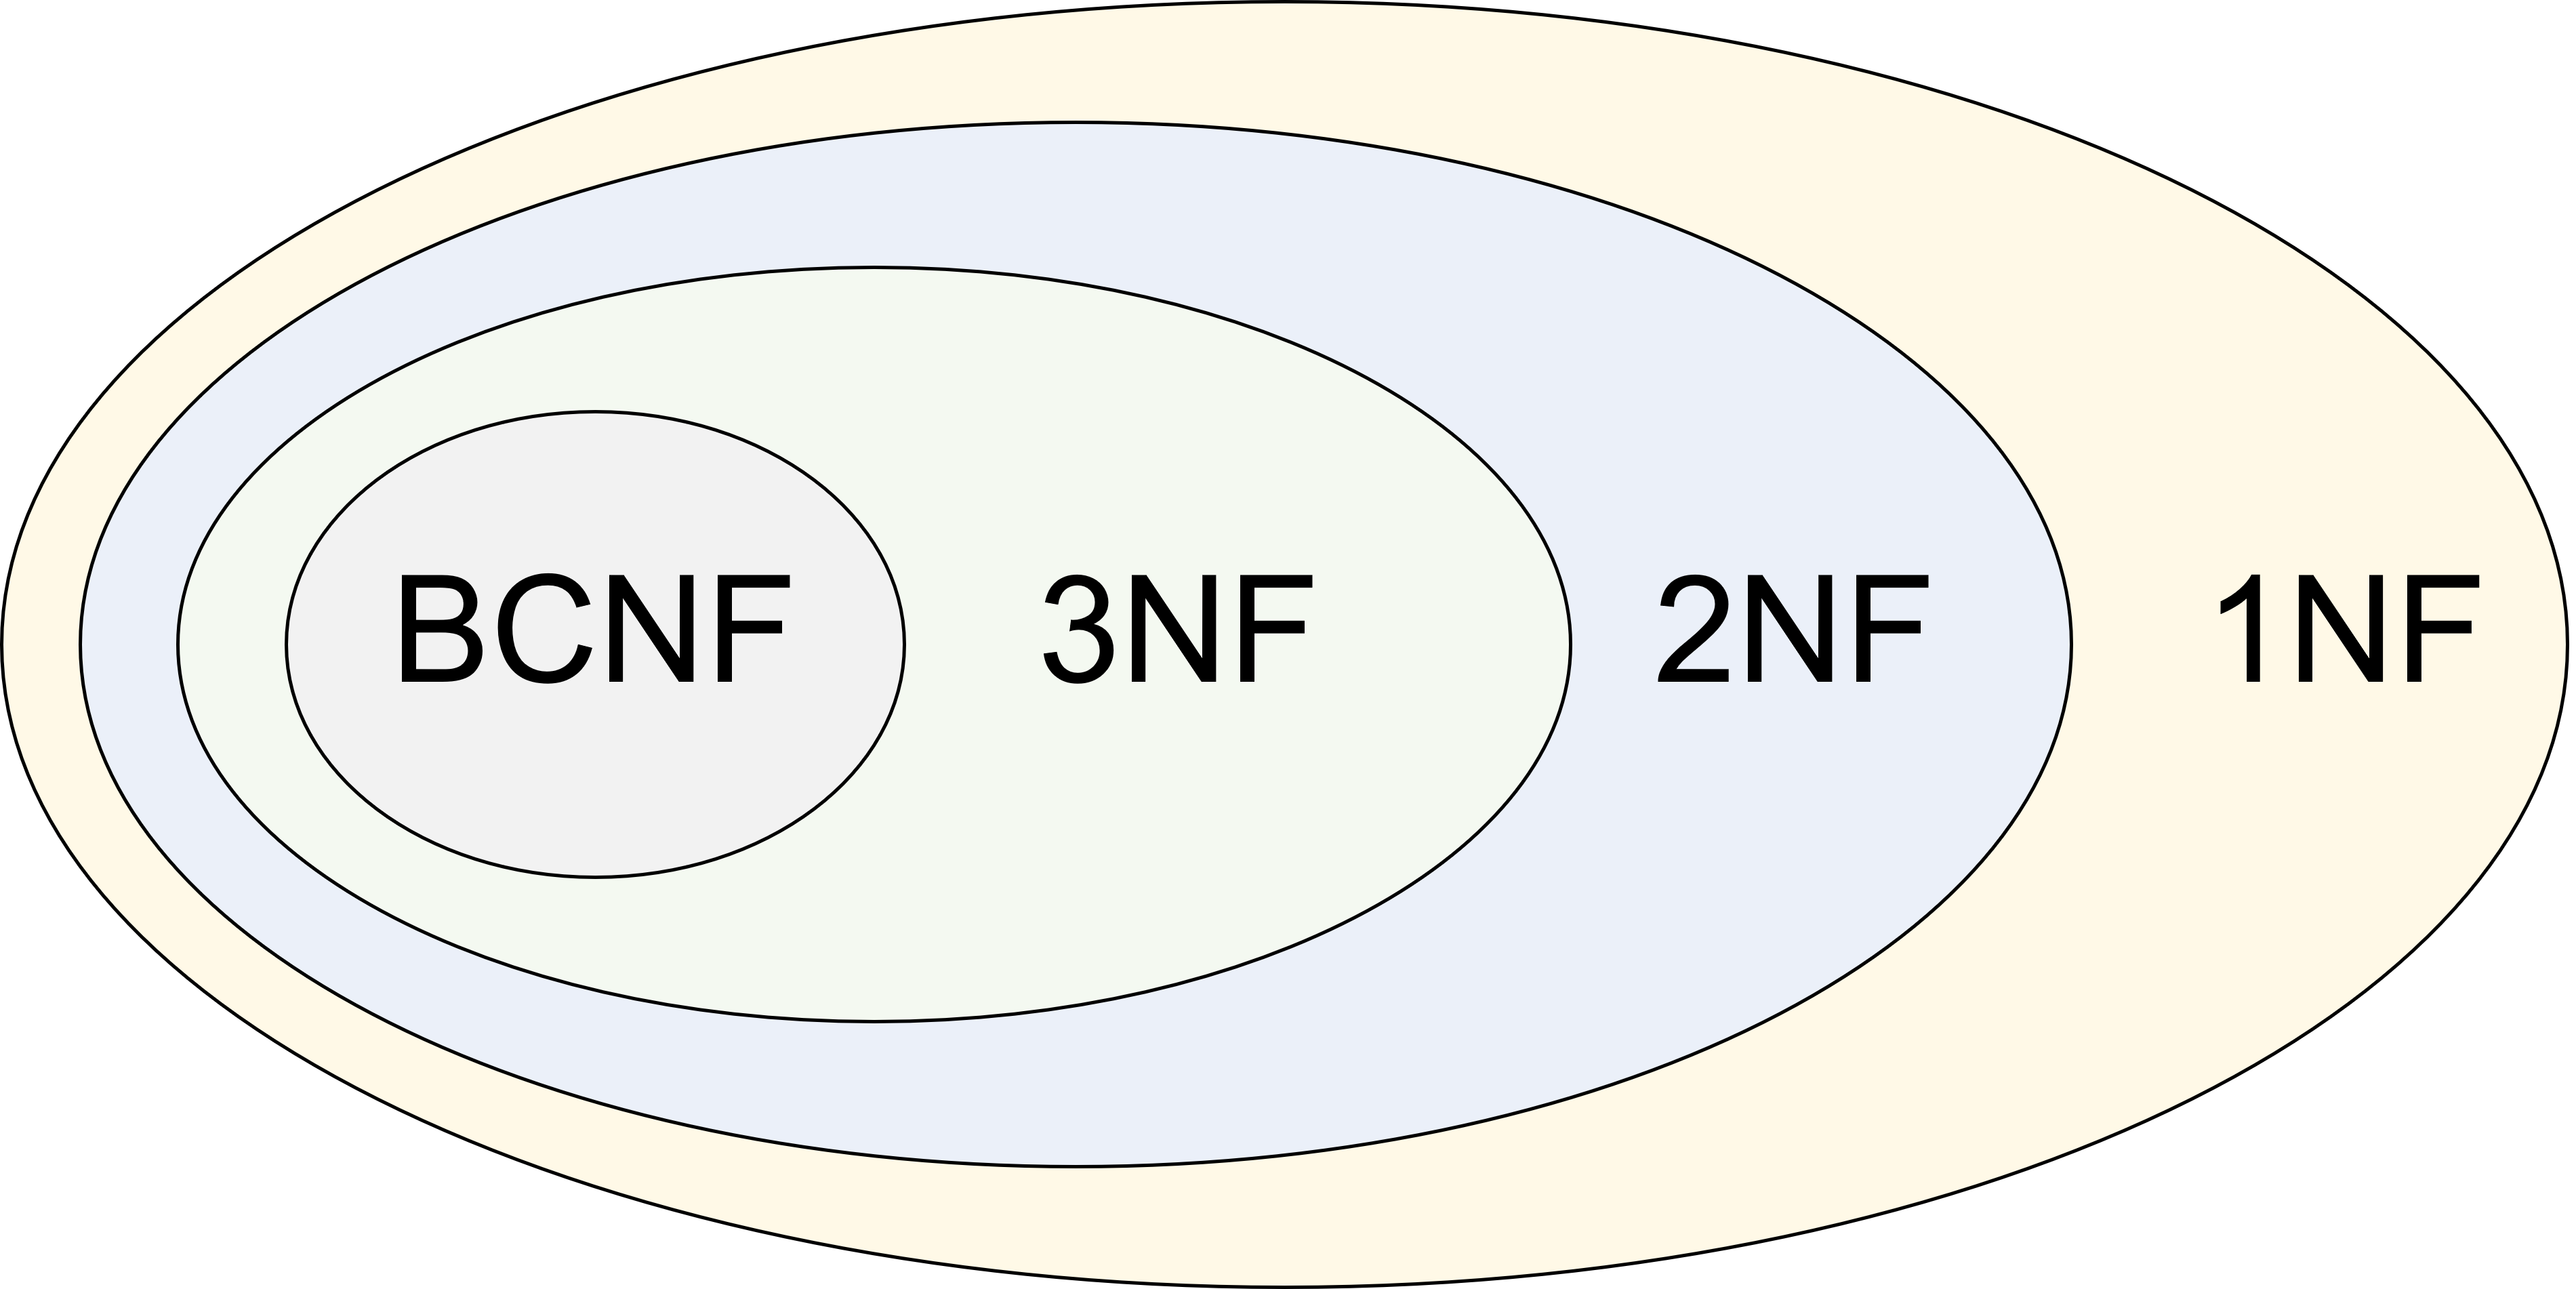
\includegraphics[width=0.75\textwidth, trim=0 0 0 0, clip]{t5/images/normal_forms.png}
\end{figure}
\end{frame}

\begin{frame}[fragile]{Question 1 (b-c) Cont.}
(*) Is $R$ with $\Sigma$ in 2NF?\\\vspace{10pt}

\textbf{Recap}: How to \textcolor{brown}{mechanically} define 2NF?\\\vspace{10pt}
A relation $R$ with a set of functional dependencies $\Sigma$ is in second norm form (2NF) if and only iff for every functional dependency $X\rightarrow\{A\}$, we have:
\begin{itemize}
	\item $X\rightarrow\{A\}$ is trivial, or
	\item $X$ is not a subset of a candidate key, or
	\item $A$ is a prime attribute.
\end{itemize}\vspace{10pt}

\begin{alertblock}{Just to understand, no need to keep it in mind!}
	Unlike the 1NF that allow any attribute as long as they are single values, 
	The 2NF is more strict so that it does not allow any non-prime attribute to be determined by partial (not full) candidate keys.
\end{alertblock}

\end{frame}

\begin{frame}[fragile]{Question 1 (b-c) Cont.}
\begin{figure}
	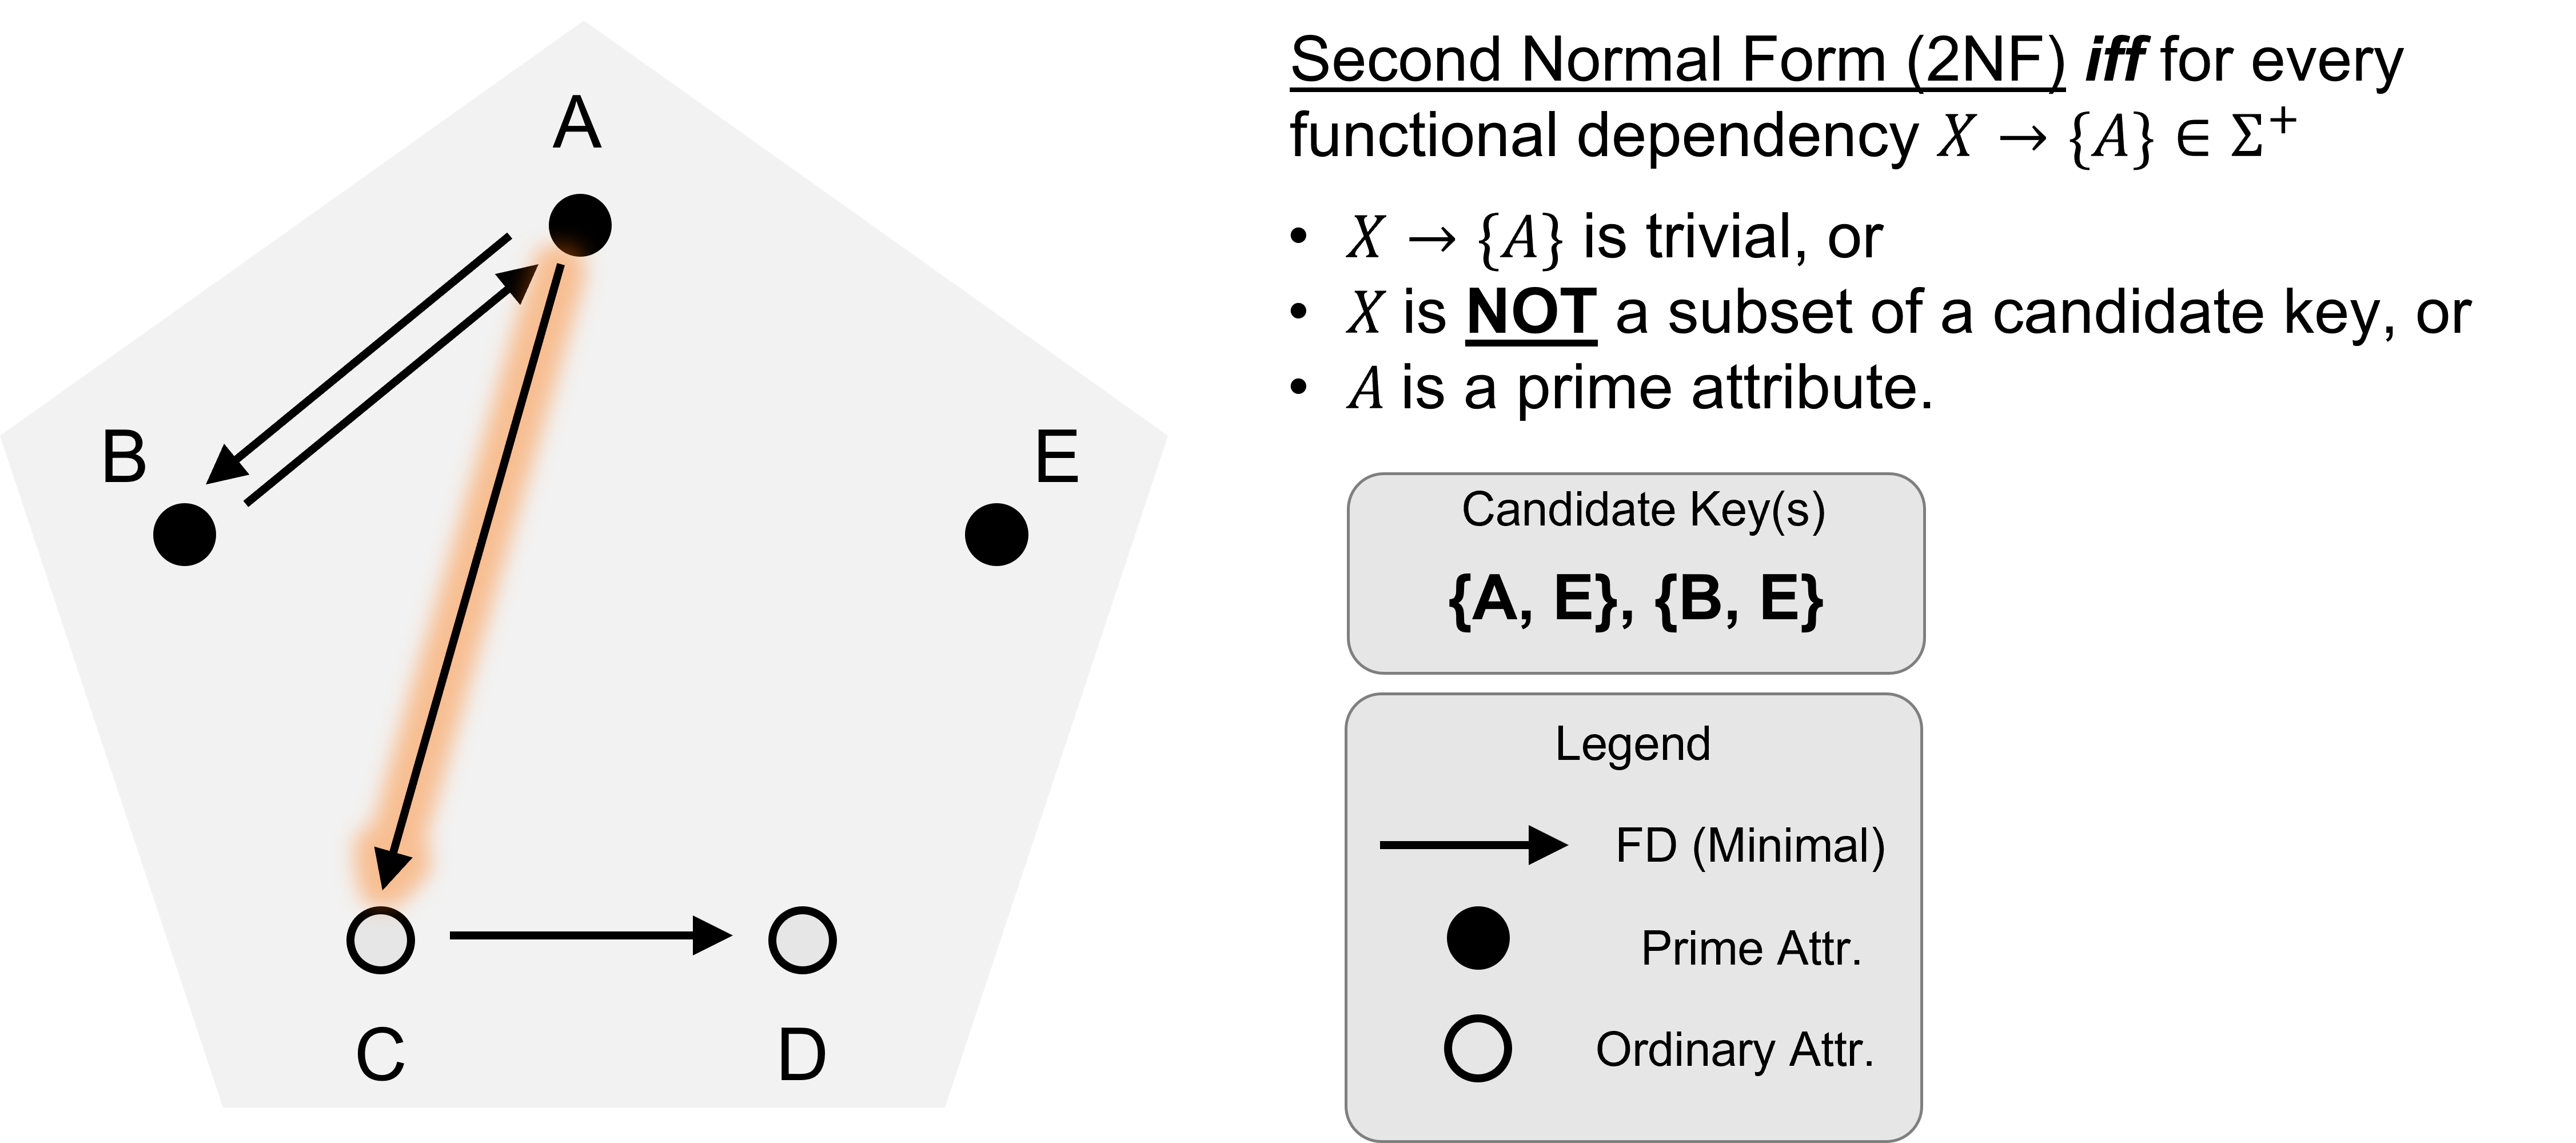
\includegraphics[width=0.85\textwidth, trim=0 0 0 0, clip]{t5/images/q3_2nf_highlight.png}
\end{figure}
\end{frame}

\begin{frame}[fragile]{Question 1 (b-c) Cont.}
\textbf{Solution}:
Let us look at the non-trivial functional dependencies of the form $X \rightarrow \{A\}$ derived from $\Sigma$. Namely after removing the trivial functional dependencies after step 1 of the minimal cover algorithm. Equivalently, we could use a minimal cover.\\\vspace{3pt}
$\{A\} \rightarrow \{C\}$ is non-trivial, $\{A\}$ is a proper subset of a candidate key and $\{C\}$ is not a prime attribute. This functional dependency violates the three conditions of the 2NF definition. $R$ with $\Sigma$ is not in 2NF.\\\vspace{3pt}

Incidentally, several other functional dependencies also violate the 2NF definition:\\
$\{B\} \rightarrow \{C\}$ is non-trivial, $\{B\}$ is a proper subset of a candidate key and $\{C\}$ is not a prime attribute. \\\vspace{3pt}
This ones do not (one condition is met):\\
$\{B,C\} \rightarrow \{D\}$ $\{B,C\}$ is not a proper subset of a candidate key.\\
$\{C\} \rightarrow \{D\}$ $\{C\}$ is not a proper subset of a candidate key.\\
$\{A\} \rightarrow \{B\}$ $\{B\}$ is a prime attribute.\\
$\{B, C\} \rightarrow \{A\}$ $\{A\}$ is a prime attribute.
\end{frame}

\begin{frame}[fragile]{Question 1 (b-c) Cont.}

(b) Is $R$ with $\Sigma$ in 3NF?\\\vspace{10pt}

\textbf{Recap}: How to \textcolor{brown}{mechanically} define 3NF?\\\vspace{10pt}
A relation $R$ with a set of functional dependencies $\Sigma$ is in third norm form (3NF) if and only iff for every functional dependency $X\rightarrow\{A\}$, we have:
\begin{itemize}
	\item $X\rightarrow\{A\}$ is trivial, or
	\item $X$ is a superkey, or
	\item $A$ is a prime attribute.
\end{itemize}\vspace{5pt}

\begin{alertblock}{Just to understand, no need to keep it in mind!}
	Unlike the 2NF that still allows a non-prime attribute to be determined by another non-prime attribute.\\ 
	The 3NF is more strict so that it does not allow any non-prime attribute to be determined by other non-prime attributes (all non-prime attributes have to be independent to each other, and therefore can only be determined by prime attributes).
\end{alertblock}

\end{frame}

\begin{frame}[fragile]{Question 1 (b-c) Cont.}
\begin{figure}
	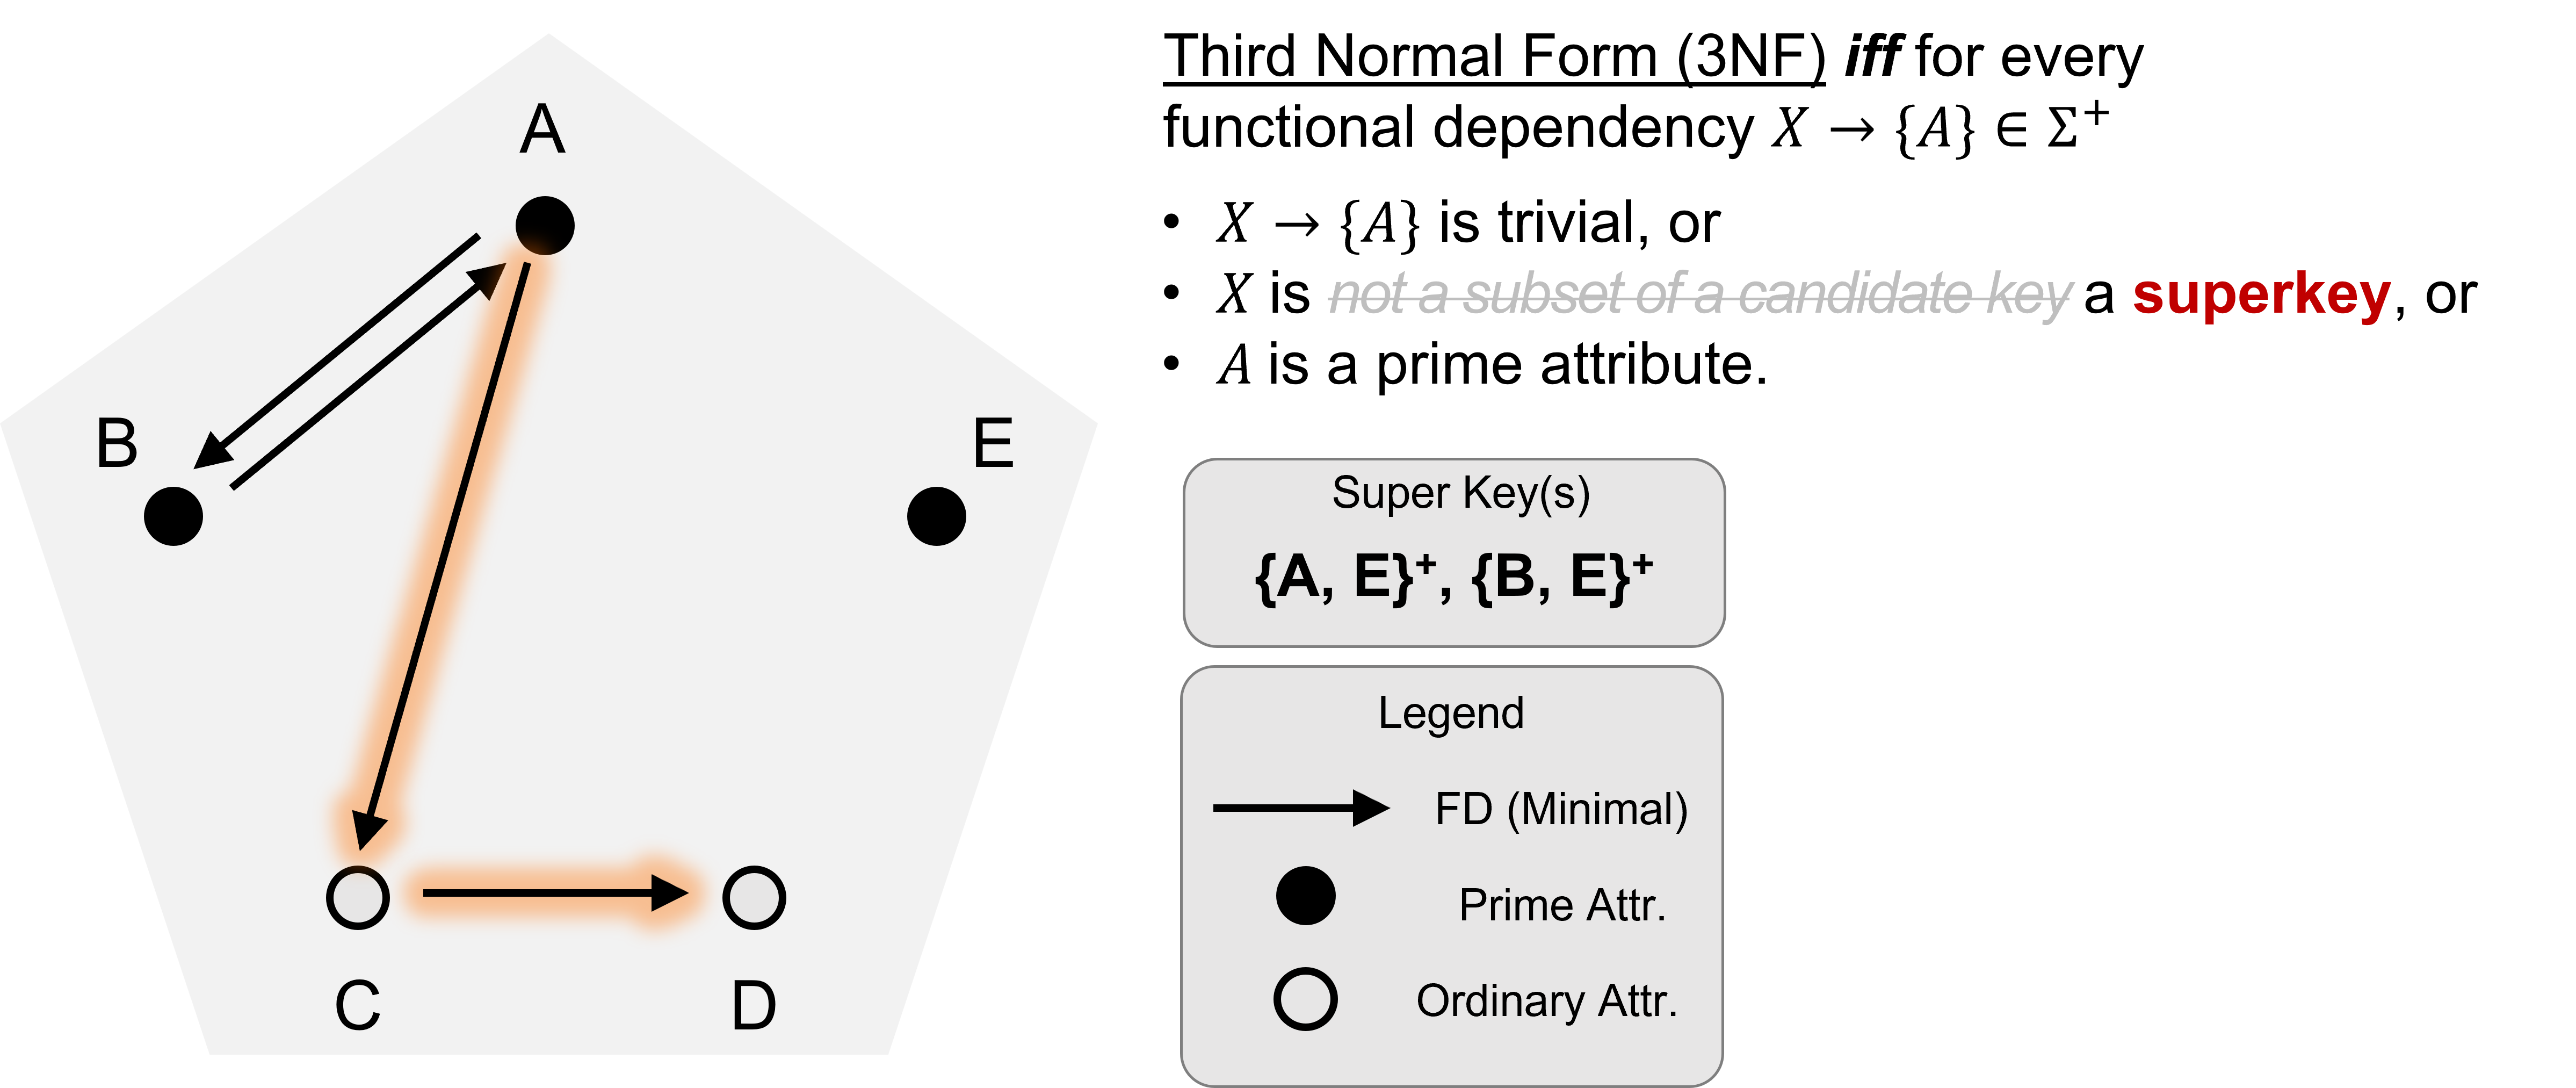
\includegraphics[width=0.95\textwidth, trim=0 0 0 0, clip]{t5/images/q3_3nf_highlight.png}
\end{figure}
\end{frame}

\begin{frame}[fragile]{Question 1 (b-c) Cont.}
\textbf{Solution}:
Let us look at the non-trivial functional dependencies of the form $X \rightarrow \{A\}$ derived from $\Sigma$. Namely after removing the trivial functional dependencies after step 1 of the minimal cover algorithm. Equivalently, we could use a minimal cover.\\\vspace{3pt}
$\{A\} \rightarrow \{C\}$ is non-trivial, $\{A\}$ is not a superkey and $\{C\}$ is not a prime attribute. This functional dependency violates the three conditions of the 3NF definition. $R$ with $\Sigma$ is not in 3NF.\\\vspace{3pt}

\end{frame}

\begin{frame}[fragile]{Question 1 (b-c) Cont.}
Incidentally, several other functional dependencies also violate the 3NF definition:\\

$\{B, C\} \rightarrow \{D\}$ is non-trivial, $\{B, C\}$ is not a superkey and $\{D\}$ is not a prime attribute.\\
$\{B\} \rightarrow \{C\}$ is non-trivial, $\{B\}$ is not a superkey and $\{C\}$ is not a prime attribute.\\
$\{C\} \rightarrow \{D\}$ is non-trivial, $\{C\}$ is not a superkey and $\{D\}$ is not a prime attribute.\\\vspace{10pt}

This two do not (one condition is met):\\
$\{A\} \rightarrow \{B\}$ is non-trivial, $\{A\}$ is not a superkey but $\{B\}$ is a prime attribute.\\\vspace{3pt}
$\{B, C\} \rightarrow \{A\}$ $\{A\}$ is a prime attribute.\\\vspace{3pt}

\end{frame}

\begin{frame}[fragile]{Question 1 (b-c) Cont.}
(c) Is $R$ with $\Sigma$ in BCNF?\\\vspace{10pt}

\textbf{Recap}: How to \textcolor{brown}{mechanically} define BCNF?\\\vspace{10pt}
A relation $R$ with a set of functional dependencies $\Sigma$ is in Boyce-Codd norm form (BCNF) if and only iff for every functional dependency $X\rightarrow\{A\}$, we have:
\begin{itemize}
	\item $X\rightarrow\{A\}$ is trivial, or
	\item $X$ is a superkey.
\end{itemize}\vspace{3pt}

\begin{alertblock}{Just to understand, no need to keep it in mind!}
BCNF was proposed in 1974 (3 years later than 2NF and 3NF) and was known as 3.5NF at the beginning.\\\vspace{3pt}
Unlike the 3NF that does not allow a non-prime attribute to be determined by other non-prime attributes (e.g. \texttt{city} is determined by \texttt{postal} in a database that record residence details). 
The BCNF is more strict so that it only allow attribute(s) to be determined by superkeys.
\end{alertblock}

\end{frame}

\begin{frame}[fragile]{Question 1 (b-c) Cont.}
\begin{figure}
	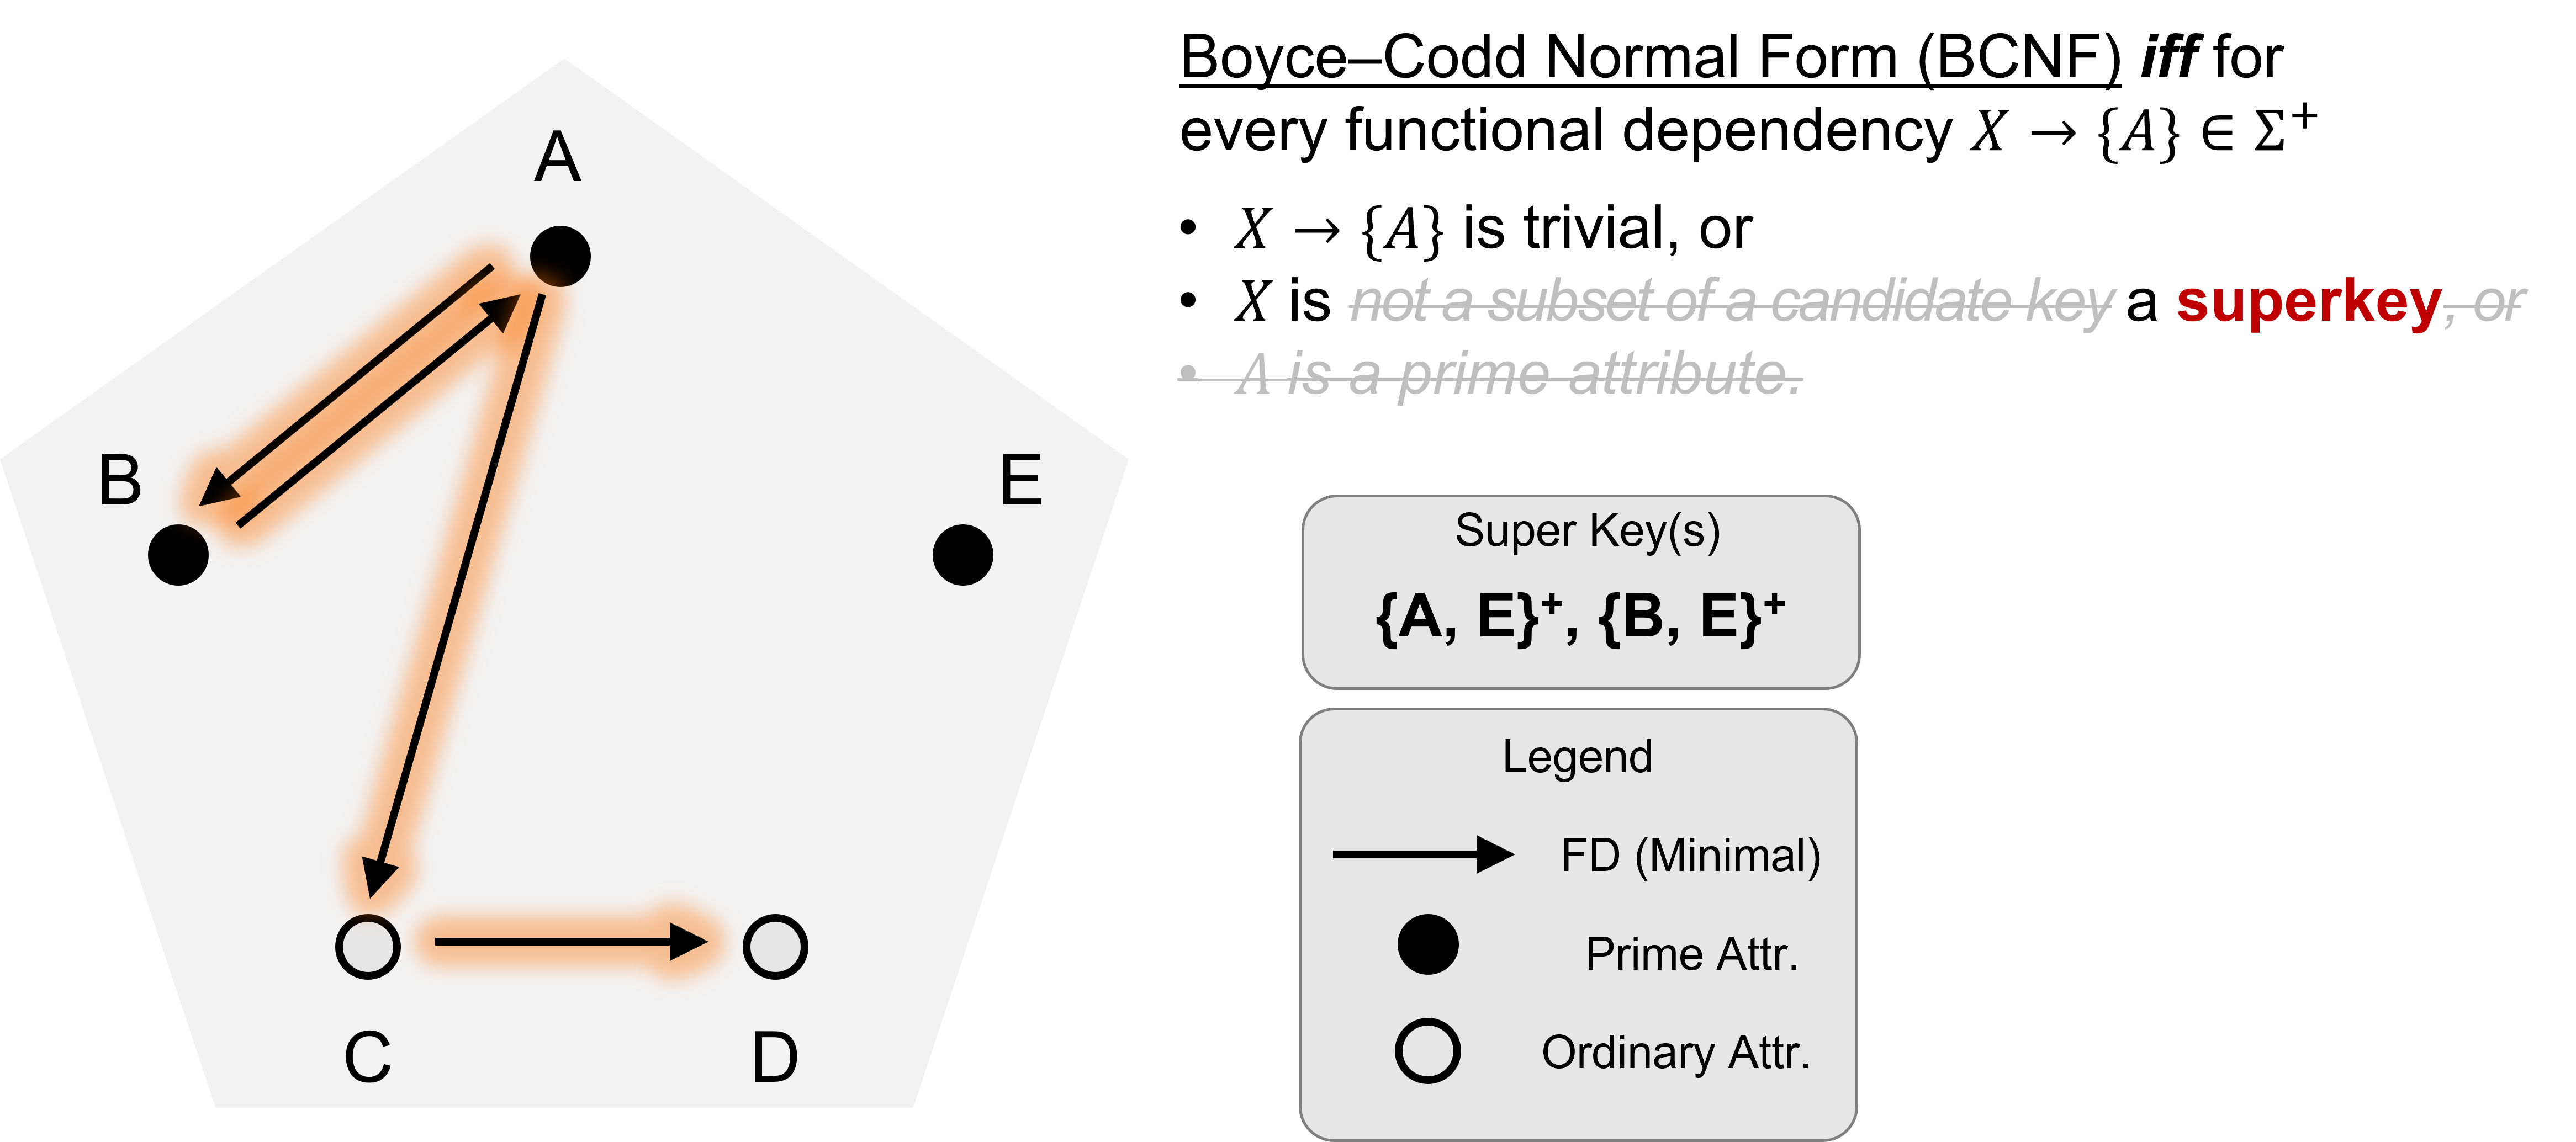
\includegraphics[width=0.85\textwidth, trim=0 0 0 0, clip]{t5/images/q3_bcnf_highlight.png}
\end{figure}
\end{frame}

\begin{frame}[fragile]{Question 1 (b-c) Cont.}
\textbf{Solution}:
$R$ with $\Sigma$ is not in 3NF, then it cannot be in BCNF.\\\vspace{3pt}

Let us look at the non-trivial functional dependencies of the form $X \rightarrow \{A\}$ derived from $\Sigma$. Namely after removing the trivial functional dependencies after step 1 of the minimal cover algorithm. Equivalently, we could use a minimal cover.\\\vspace{3pt}

$\{A\} \rightarrow \{C\}$ is non-trivial and $\{A\}$ is not a superkey . This functional dependency violates the two conditions of the BCNF definition. $R$ with $\Sigma$ is not in BCNF.\\\vspace{3pt}

Incidentally, all the other functional dependencies also violate the BCNF definition:\\
$\{A\} \rightarrow \{B\}$ is non-trivial and $\{A\}$ is not a superkey.\\
$\{B, C\} \rightarrow \{D\}$ is non-trivial and $\{B, C\}$ is not a superkey.\\
$\{B\} \rightarrow \{C\}$ is non-trivial and $\{B\}$ is not a superkey.\\
$\{C\} \rightarrow \{D\}$ is non-trivial and  $\{C\}$ is not a superkey.\\
$\{B, C\} \rightarrow \{A\}$ $\{A\}$ is non-trivial and  $\{B, C\}$ is not a superkey.
\end{frame}

\begin{frame}[fragile]{Question 1 (d-j) Normalisation}
	(d) Decompose $R$ with $\Sigma$ into a BCNF decomposition using the algorithm from the lecture.\\\vspace{5pt}
	
	\textbf{Solution}: We found that $\{A\} \rightarrow \{C\}$ violates the BCNF condition.\\\vspace{3pt}
	
	We use it to decompose into two fragments:\\
	$R_1 = \{A\}^{+} = \{A, B, C, D\}$ with $\Sigma_1 = \{\{A\} \rightarrow \{C\}, \{A\} \rightarrow \{B\},\{B\} \rightarrow \{A\}, \{C\} \rightarrow \{D\}\}$.
	
	$R_2 = \{A, E\}$ with $\Sigma_2 = \emptyset$.
	
	$R_2$ with $\Sigma_2$ is in BCNF.
	
	$R_1$ with $\Sigma_1$ is not in BCNF because $\{C\} \rightarrow \{D\}$ violates the BCNF condition.
	\textbf{$\leftarrow$ We need to further decompose it.}
\end{frame}

\begin{frame}[fragile]{Question 1 (d-j) Cont.}
	For $R_1 = \{A\}^{+} = \{A, B, C, D\}$, we use it to decompose into two fragments:\\\vspace{5pt}
	$R_{1.1} = \{C\}^{+} = \{C, D\}$ (computed for $R_1$ with $\Sigma_1$!) with $\Sigma_{1.1} = \{\{C\} \rightarrow \{D\}\}$.
	
	$R_{1.2} = \{A, B, C\}$ with $\Sigma_{1.2} = \{\{A\} \rightarrow \{B\}, \{A\} \rightarrow \{C\}, \{B\} \rightarrow \{A\}\}$.\\\vspace{5pt}
	
	$R_{1.1}$ with $\Sigma_{1.1}$ is in BCNF.
	
	$R_{1.2}$ with $\Sigma_{1.2}$ is in BCNF.\\\vspace{5pt}
	
	The result is a decomposition into three fragments: $R_2$, $R_{1.1}$ and $R_{1.2}$.\\\vspace{5pt}
\end{frame}

\begin{frame}[fragile]{Question 1 (d-j) Cont.}
	(e) Is the results lossless?\\\vspace{5pt}
	\textbf{Solution}: Yes, the algorithm guarantees that the result is lossless.\\
	\vspace{30pt}
	(f) Is the results dependency preserving?\\\vspace{5pt}
	\textbf{Solution}:
	Incidentally yes, the \textbf{algorithm} (itself) \textcolor{red}{\textbf{does not}} guarantee that the result is dependency preserving.\\
	\begin{alertblock}{Notice}
		Don't take the dependency preserving for granted in decomposition.
	\end{alertblock}
	
\end{frame}

\begin{frame}[fragile]{Question 1 (d-j) Cont.}
(g) Synthesise $R$ with $\Sigma$ into a 3NF decomposition using the algorithm from the lecture.\\\vspace{5pt}

\textbf{Solution}:
First compute a compact minimal cover:

$\{A\} \rightarrow \{B, C\}$

$\{B\} \rightarrow \{A\}$

$\{C\} \rightarrow \{D\}$

For each functional dependency create a fragment:

$R_1 = \{A, B, C\}$

$R_2 = \{B, A\}$ , this fragment is not kept: it is subsumed by $R_1$.

$R_3 = \{C, D\}$.

None of the fragments contain a candidate key. We choose one: say $\{A, E\}$, and add it as fragment:

$R_4 = \{A, E\}$.

The result is:
$R_1 = \{\underline{A}, \underline{B}, C\}$
$R_3 = \{\underline{C}, D\}$.
$R_4 = \{\underline{A, E}\}$.

The algorithm always works. It is guaranteed to find a decomposition in 3NF. Note that using a different minimal cover or compact minimal cover may give a different (but equally correct) result.
\end{frame}

\begin{frame}[fragile]{Question 1 (d-j) Cont.}
(h) Is the results lossless?\\\vspace{5pt}
\textbf{Solution}: Yes, the algorithm guarantees that the result is lossless.
\\\vspace{30pt}
(i) Is the results dependency preserving?\\\vspace{5pt}
\textbf{Solution}:
Yes, the algorithm guarantees that the result is dependency preserving.

\end{frame}

\begin{frame}[fragile]{Question 1 (d-j) Cont.}
(j) Is the results in BCNF?\\\vspace{5pt}

\textbf{Solution}:
The algorithm guarantees that the result is in 3NF. In this case, it is also in BCNF! (you can check). It is not always but often the case.\\\vspace{10pt}

\textcolor{red}{\textbf{Extra}}:\\
To wrap-up, BCNF decomposition is \textbf{not always optimal}, as it aims to dismiss some ``unnecessary'' dependencies among attributes. (sometimes 3NF is good enough)\\\vspace{5pt}
\end{frame}

\begin{comment}
	
\section*{Extra Practice}

\begin{frame}[fragile]{\boss{Extra Practice}}
	Challenging questions ahead!!! I share with you 4 practice questions and each one may cost you 5-10 mins.\\\vspace{10pt}
	\textcolor{brown}{If you can UNDERSTAND \& SOLVE them, you basically uderstand all key knowledge of this tutorial and you should be fine for the exam/test.}\\\vspace{10pt}
	
	\begin{columns}[t]
	\column{0.65\textwidth}
	\\\vspace{5pt}
	\textbf{Free lunch, Die-die must try!}\\\vspace{10pt}
	(Due to time limitation, solutions will be posted on Luminus and elaborated right after zoom TG10 session (Fri 9:30 PM onwards). You can feel free to join the TG10 zoom or watch the video recording later)
	\column{0.25\textwidth}
	\begin{figure}
		
\includegraphics[width=1\textwidth, trim=0 0 0 0, clip]{t5/images/mario.png}
	\end{figure}
\end{columns}
\end{frame}

\end{comment}
% \begin{comment}
\begin{frame}[fragile]{\boss{Extra Exercise}}
	There are four extra exercises for you to practice what have learned in normalisation lecture. 
	As normalisation is one of the most challenging parts of the fundamental database module, it would be helpful for you to evaluate your understanding of this part. \\
\end{frame}
\end{comment}

\begin{frame}[fragile]{\boss{Extra} - Case 1}
	We are designing a warehouse management system for a lot of warehouses. Each warehouse ($W$) has one manager ($M$), and each manager only manage one warehouse. There could be many products ($P$) in per warehouse. For each product we also record its stock number ($S$).\\\vspace{10pt}
	\textbf{Questions}:\\
	(1) Find \textbf{candidate key(s)} and \textbf{prime attribute(s)} from attribute closures $\Sigma^{+}$.\\
	(2) Compute the \textbf{compact minimal cover} of $R$ with all FDs $\Sigma$.\\
	(3) Determine if it is \textbf{2NF}? If yes, is it \textbf{3NF}? If yes, is it \textbf{BCNF}?\\
	(4) If it is not 3NF, \textbf{synthesis} the relations to make it 3NF.\\
	(5) If it is not BCNF, \textbf{decomposite} the relations to make it BCNF and verify the \textbf{dependency preservation}. 
\end{frame}

\begin{frame}[fragile]{\boss{Extra} - Case 2}
	We are designing a transcript issuing system for our university. 
	Each student is identified by its matric number/student ID, written as $S$.
	We are going to record a grade ($G$) for each student ($S$) and each module ($M$).
	We also record students' names ($N$) and their faculty ($F$). In case any verification is needed, we also save the dean's name for each department ($D$) so that people can contact him/her.\\\vspace{10pt}
	\textbf{Questions}:\\
	(1) Find \textbf{candidate key(s)} and \textbf{prime attribute(s)} from attribute closures $\Sigma^{+}$.\\
	(2) Compute the \textbf{compact minimal cover} of $R$ with all FDs $\Sigma$.\\
	(3) Determine if it is \textbf{2NF}? If yes, is it \textbf{3NF}? If yes, is it \textbf{BCNF}?\\
	(4) If it is not 3NF, \textbf{synthesis} the relations to make it 3NF.\\
	(5) If it is not BCNF, \textbf{decomposite} the relations to make it BCNF and verify the \textbf{dependency preservation}. 
\end{frame}

\begin{frame}[fragile]{\boss{Extra} - Case 3}
	This time we deal with abstract relations with functional dependencies shown as in the figure below:\\\vspace{-5pt}
	
	\begin{figure}
		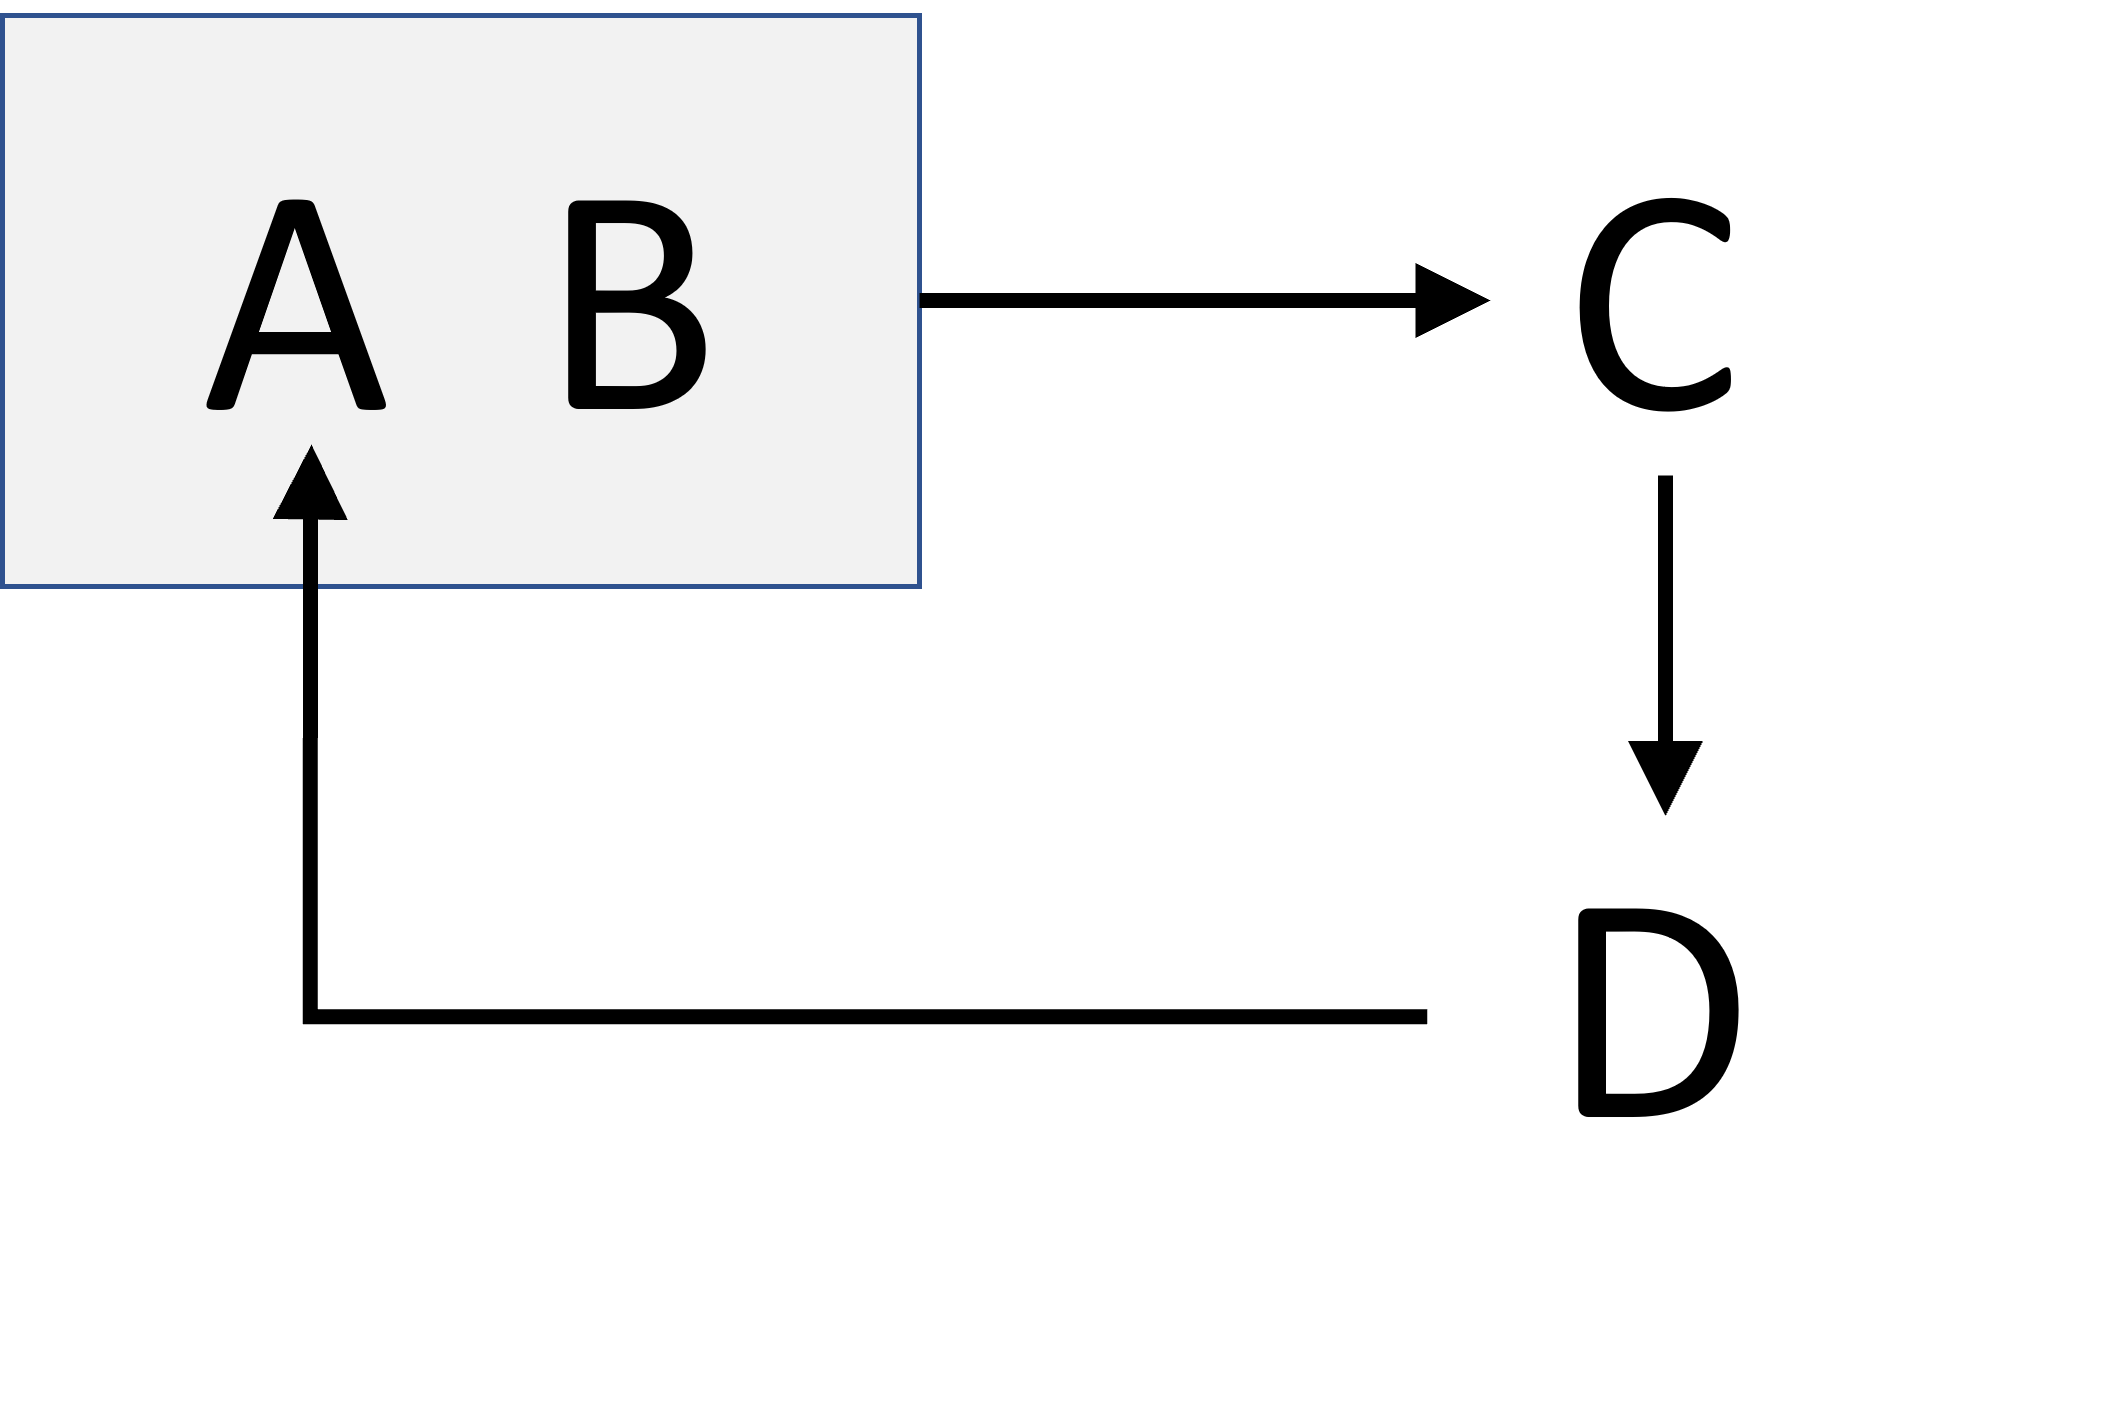
\includegraphics[width=0.4\textwidth, trim=0 0 0 0, clip]{t5/images/case3.png}
	\end{figure}\vspace{-10pt}
	
	\textbf{Questions}:\\
	(1) Find \textbf{candidate key(s)} and \textbf{prime attribute(s)} from attribute closures $\Sigma^{+}$.\\
	(2) Compute the \textbf{compact minimal cover} of $R$ with all FDs $\Sigma$.\\
	(3) Determine if it is \textbf{2NF}? If yes, is it \textbf{3NF}? If yes, is it \textbf{BCNF}?\\
	(4) If it is not 3NF, \textbf{synthesis} the relations to make it 3NF.\\
	(5) If it is not BCNF, \textbf{decomposite} the relations to make it BCNF and verify the \textbf{dependency preservation}. 
\end{frame}

\begin{frame}[fragile]{\boss{Extra} - Case 4}
	Another abstract relations with functional dependencies shown as in the figure below:\\\vspace{-5pt}
	
	\begin{figure}
		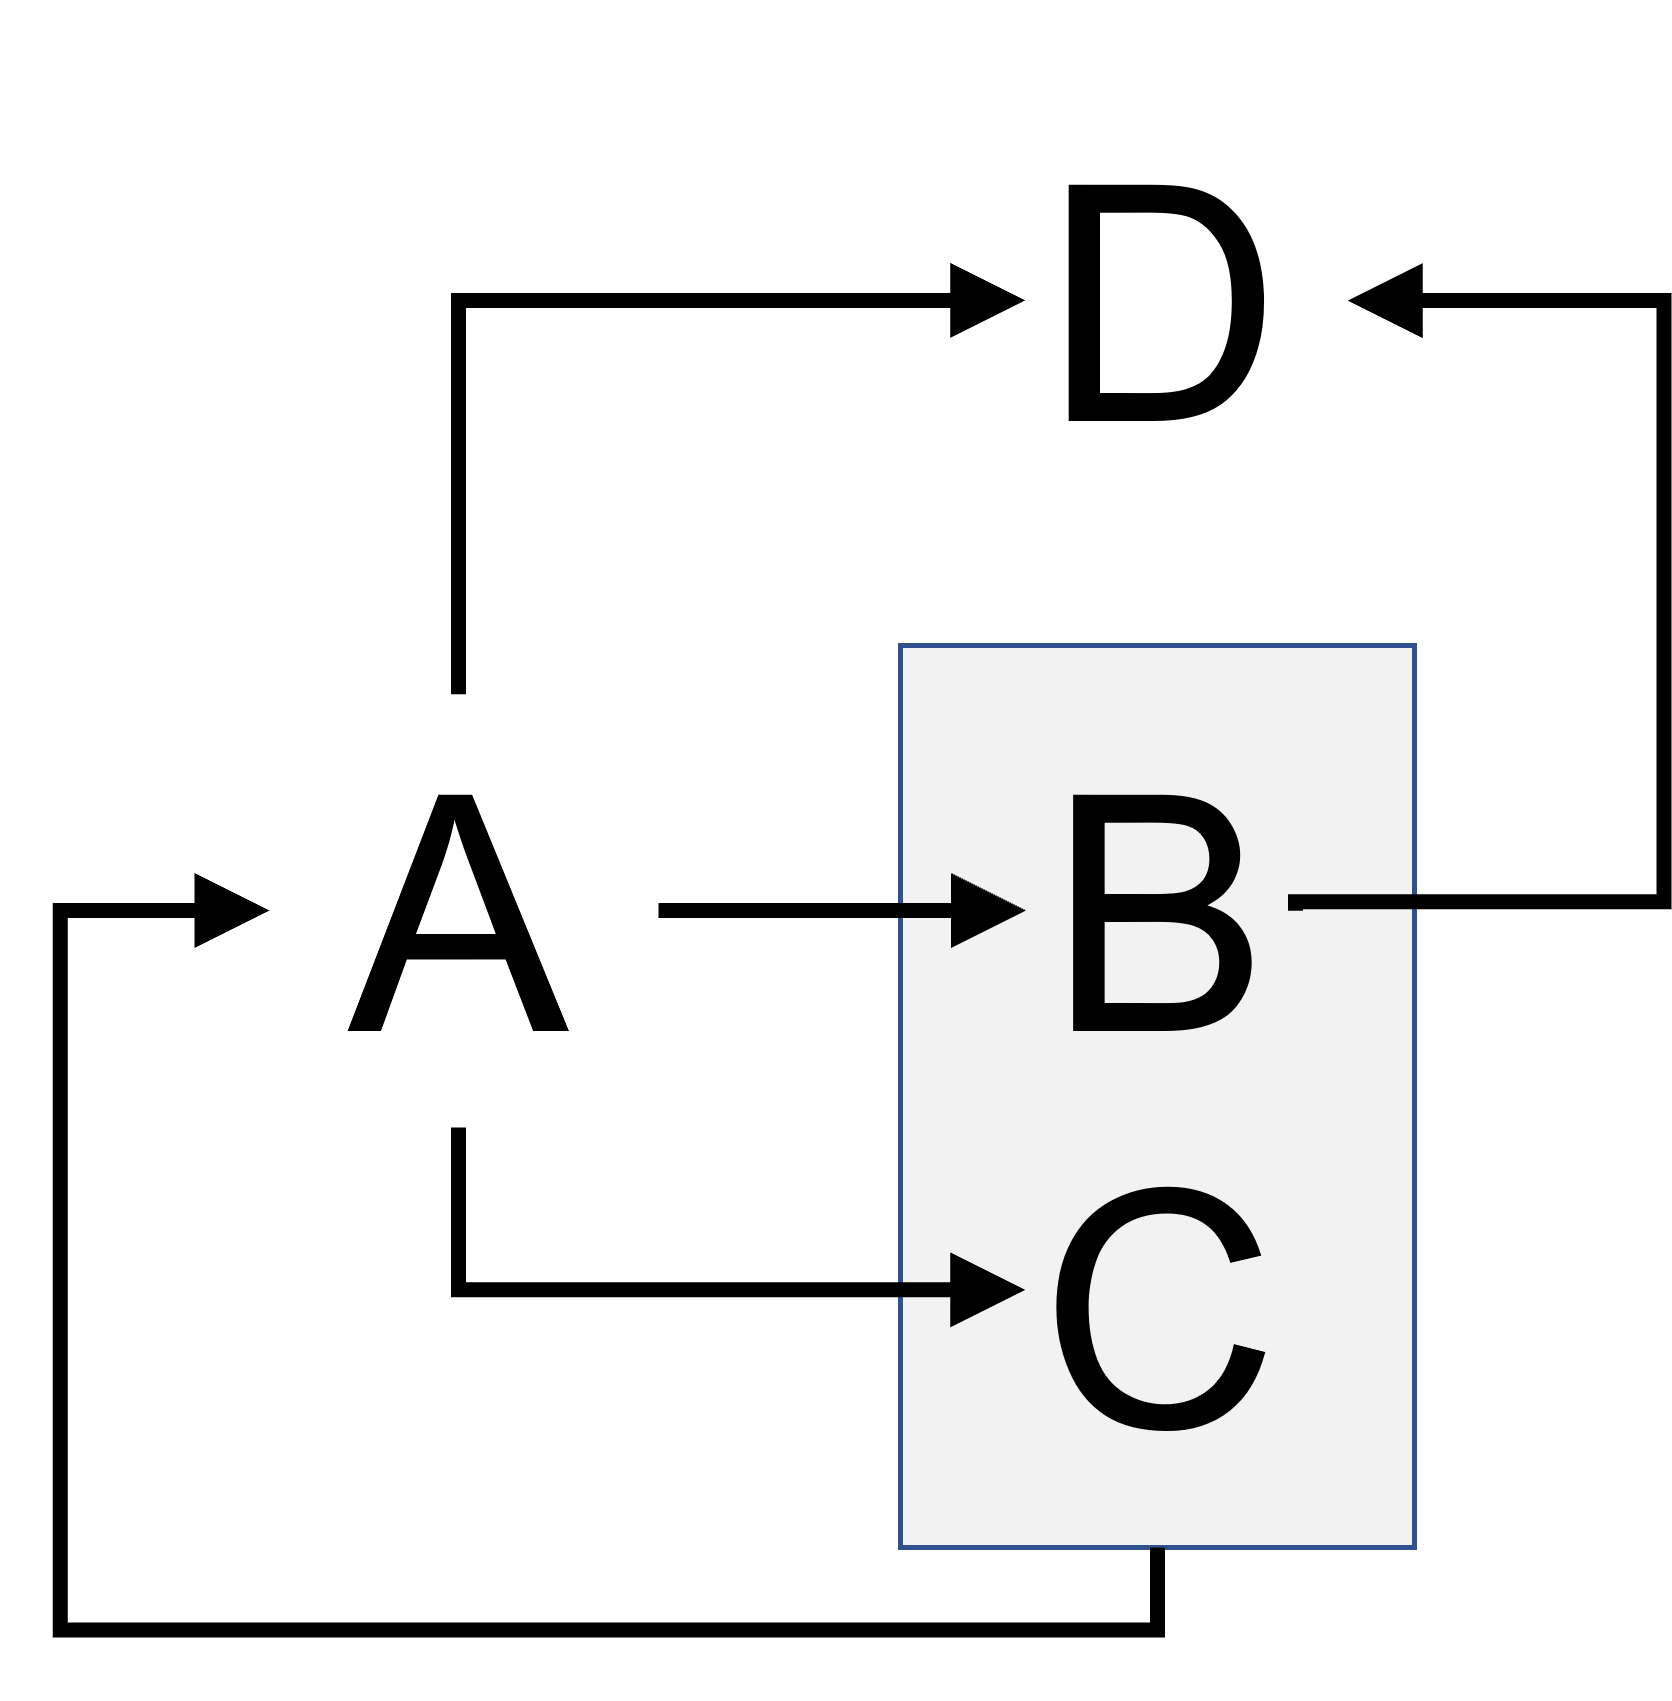
\includegraphics[width=0.25\textwidth, trim=0 0 0 0, clip]{t5/images/case4.png}
	\end{figure}\vspace{-5pt}
	
	\textbf{Questions}:\\
	(1) Find \textbf{candidate key(s)} and \textbf{prime attribute(s)} from attribute closures $\Sigma^{+}$.\\
	(2) Compute the \textbf{compact minimal cover} of $R$ with all FDs $\Sigma$.\\
	(3) Determine if it is \textbf{2NF}? If yes, is it \textbf{3NF}? If yes, is it \textbf{BCNF}?\\
	(4) If it is not 3NF, \textbf{synthesis} the relations to make it 3NF.\\
	(5) If it is not BCNF, \textbf{decomposite} the relations to make it BCNF and verify the \textbf{dependency preservation}. 
\end{frame}



\begin{frame}{}
	\begin{figure}
		
\includegraphics[width=0.6\textwidth, trim=0 3.5cm 0 0, clip]{t5/images/final.png}
	\end{figure}
\begin{center}
	Enjoy the recess week and have a good rest. Keep safe!
\end{center} 
\end{frame}
\begin{frame}{}
	\centering  
	For any further question, please feel free to email me:\vspace{10pt}
	
	huasong.meng@u.nus.edu\\\vspace{3pt}
	%menghs@i2r.a-star.edu.sg (work)\\\vspace{3pt}
	%huasong.meng@gmail.com (personal)\vspace{10pt}
	
	Or you can whatsapp/wechat me via: 81028639 \vspace{20pt}
	
	\begin{tcolorbox}
		\begin{center}
			\textcolor{red}{Copyright 2021 Mark H. Meng. All rights reserved.}
		\end{center}
	\end{tcolorbox}
\end{frame}